\section{Qué pasó en el entrenamiento}

\begin{figure}[H]
\centering
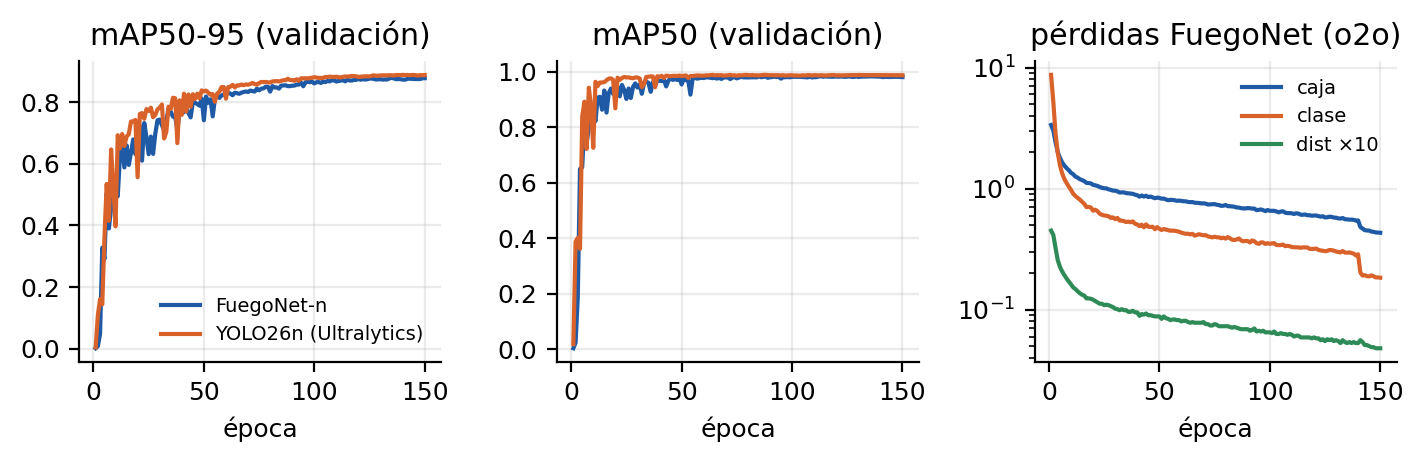
\includegraphics[width=\textwidth]{curvas.png}
\caption{Entrenamiento desde cero. Izquierda y centro: mAP en validación de
FuegoNet-n (este manual) y de YOLO26n de Ultralytics con la misma receta.
Derecha: pérdidas de la cabeza o2o de FuegoNet (escala logarítmica).}
\label{fig:curvas}
\end{figure}

\begin{itemize}
  \item El entrenamiento corrió 150 épocas en 156 minutos
        (unos 62~s por época, compartiendo la
        GPU con la corrida de control).
  \item El mejor modelo (\cod{mejor.pt}) es el de la época 135: mAP50 =
        0.984 y mAP50-95 = 0.879 en validación
        (AP50-95 de fuego 0.879, de humo 0.879).
  \item En la época 10 ya tenía mAP50 = 0.859: la mayor parte se aprende
        pronto y las últimas épocas afinan las cajas (sube sobre todo el mAP50-95).
  \item Al apagar el mosaico (últimas 10 épocas) hay un salto pequeño hacia arriba: la
        red se ajusta a imágenes completas como las de vuelo.
\end{itemize}

\begin{nota}
La curva naranja es el control: YOLO26n de Ultralytics, también desde cero, con los
mismos datos y aumentos. Su mejor época (140) da mAP50-95 =
0.889 \emph{según su propio validador}. La comparación
justa, con el mismo código de métricas, está en el capítulo~\ref{cap:evaluar}.
\end{nota}
